\documentclass{beamer}


\usepackage[utf8]{inputenc}
\usepackage[american]{babel}
%\usepackage{enumerate}
\usepackage{multicol}
\usepackage{amsfonts,amsmath,amssymb,amsthm,amstext,latexsym}	
%\usepackage[inline]{enumitem}

\usepackage{hyperref}
\usepackage[absolute,overlay]{textpos}
\usepackage{xspace}
%\usepackage{subcaption}
\usepackage{array,multirow,makecell}
\usepackage{todonotes}
\usepackage{ifthen}
\usepackage{intcalc}
%\usepackage{fullpage}
\usepackage[ruled,vlined,boxed,linesnumbered,commentsnumbered]{algorithm2e}
\usepackage{subfig}
%\usepackage{paralist}
%\usepackage{listings}

\usepackage{tikz}
\usetikzlibrary{calc}
\usetikzlibrary{arrows,shapes}
\usetikzlibrary{patterns,snakes}

\newcommand{\tikzmark}[1]{\tikz[overlay,remember picture,baseline] \node [anchor=base] (#1) {};}%

\newcommand{\ema}[1]{\ensuremath{#1}\xspace}

\newcommand\scalemath[2]{\scalebox{#1}{\mbox{\ensuremath{\displaystyle #2}}}}

\newcommand<>{\red}[1]{{\color#2{red!80!black}#1}}

\usetheme{Madrid}

\author[Valentin Le Fèvre]{\red{Valentin Le Fèvre}, Leonardo Bautista-Gomez, Marc Casas, Osman Unsal\\
{\small \texttt{valentin.le-fevre@ens-lyon.fr}}}

\title{Approximating a Multi-Grid Solver}
\institute[ENS de Lyon]{ENS de Lyon, Barcelona Supercomputing Center}
\date{April 17, 2018}

\begin{document}

\begin{frame}
 \maketitle
\end{frame}

\begin{frame}{Introduction}
 
 Approximate computing: trade-off between \textbf{accuracy of result} and \textbf{execution time}.

  \pause
  \begin{itemize}
    \item Precision of a floating-point value
    \item No exact result exists (search query...)
    \item ...
  \end{itemize}
  \pause
  \begin{itemize}
   \item Skip steps in loops
   \item Branching to avoid useless computations
   \item Faulty hardware (fast adders...)
   \item ...
  \end{itemize}

\end{frame}

\begin{frame}{Introduction}
 \begin{itemize}
  \item Multi-Grid (MG) solvers~\cite{Hackbusch1991}: iterative solvers with different level of coarseness: number of evaluation points.\\
  Faster than classical method and scales well.
  \begin{figure}
  \centering
 %\resizebox{\linewidth}{4cm}{
 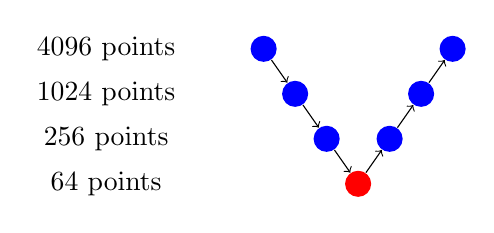
\begin{tikzpicture}
 
 
\begin{scope}[xscale=2/5,yscale=4/7]

  \node (sh) at (-8,3) { 4096 points };
  \node (shh) at (-8,2) { 1024 points };
  \node (shhh) at (-8,1) { 256 points };
  \node (shhhh) at (-8,0) { 64 points };

    \node[circle,fill=blue] (a) at (-3,3) { };
    \node[circle,fill=blue] (b) at (-2,2) {};
    \node[circle,fill=blue] (c) at (-1,1) {};
    \node[circle,fill=red] (d) at (0,0) {};
    \node[circle,fill=blue] (e) at (1,1) {};
    \node[circle,fill=blue] (f) at (2,2) {};
    \node[circle,fill=blue] (g) at (3,3) {};
    
    \draw[->] (a) -- (b);
    \draw[->] (b) -- (c);
    \draw[->] (c) -- (d);
    \draw[->] (d) -- (e);
    \draw[->] (e) -- (f);
    \draw[->] (f) -- (g);
    \end{scope}

 \end{tikzpicture}
 %}
 \caption{Example of cycle: each blue point represents one iteration of an iterative method, while the height corresponds to the coarseness of the grid. Red is ``exact`` solve.}
 
\end{figure}

\pause

\item Accuracy of result (\textit{relative residual norm}) is limited by the hardware.
\item We do not aim the same accuracy when using it as a conditioner or a solver.
 \end{itemize}
 
\end{frame}


\begin{frame}{Outline}
 \tableofcontents
\end{frame}

\section{The \textsc{Up}-cycle}

\begin{frame}{Outline}
 \tableofcontents[currentsection]
\end{frame}

\begin{frame}{Analysis}

\begin{center}
\only<1>{First idea: add more iterations at each level or more complex cycles.
    \begin{figure}
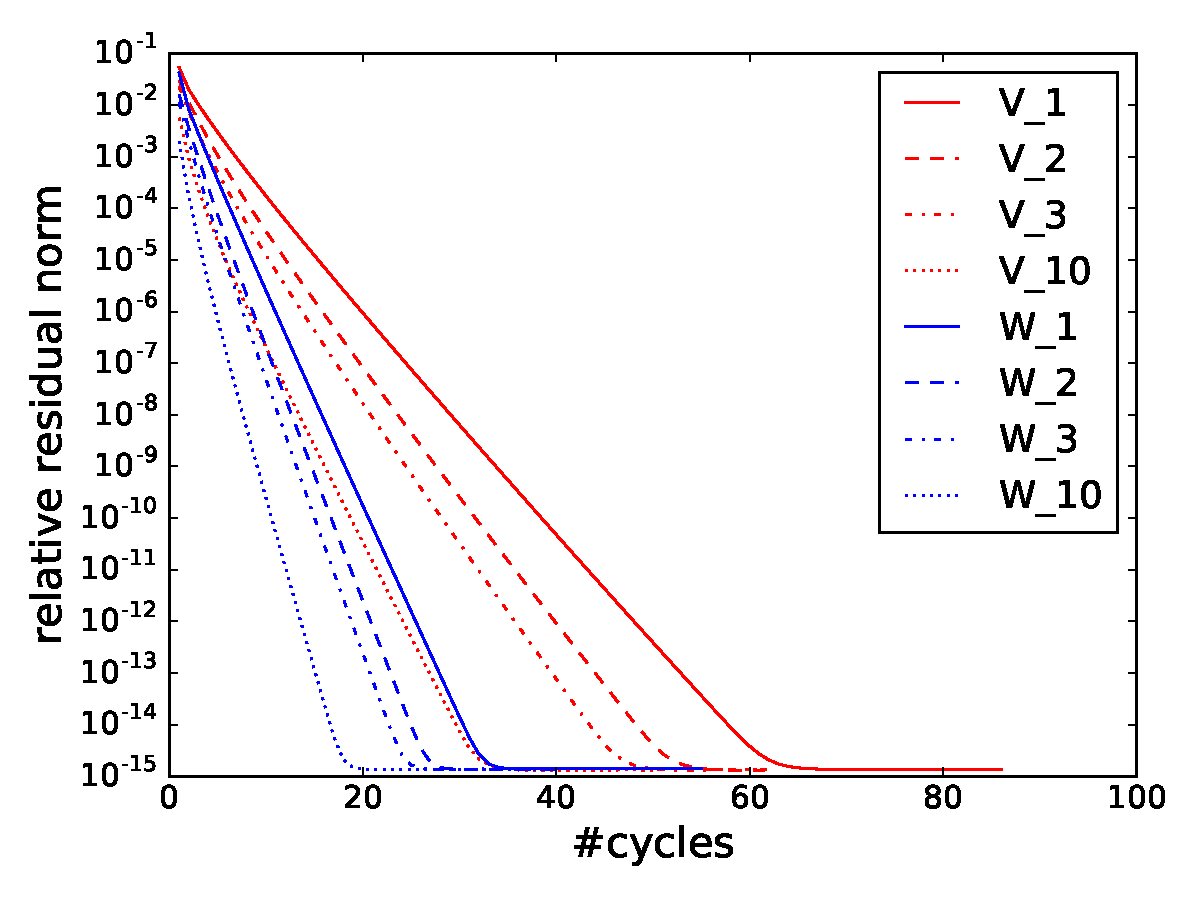
\includegraphics[width=0.4\linewidth]{../ICS/figs/convergence_1_norm.pdf}
    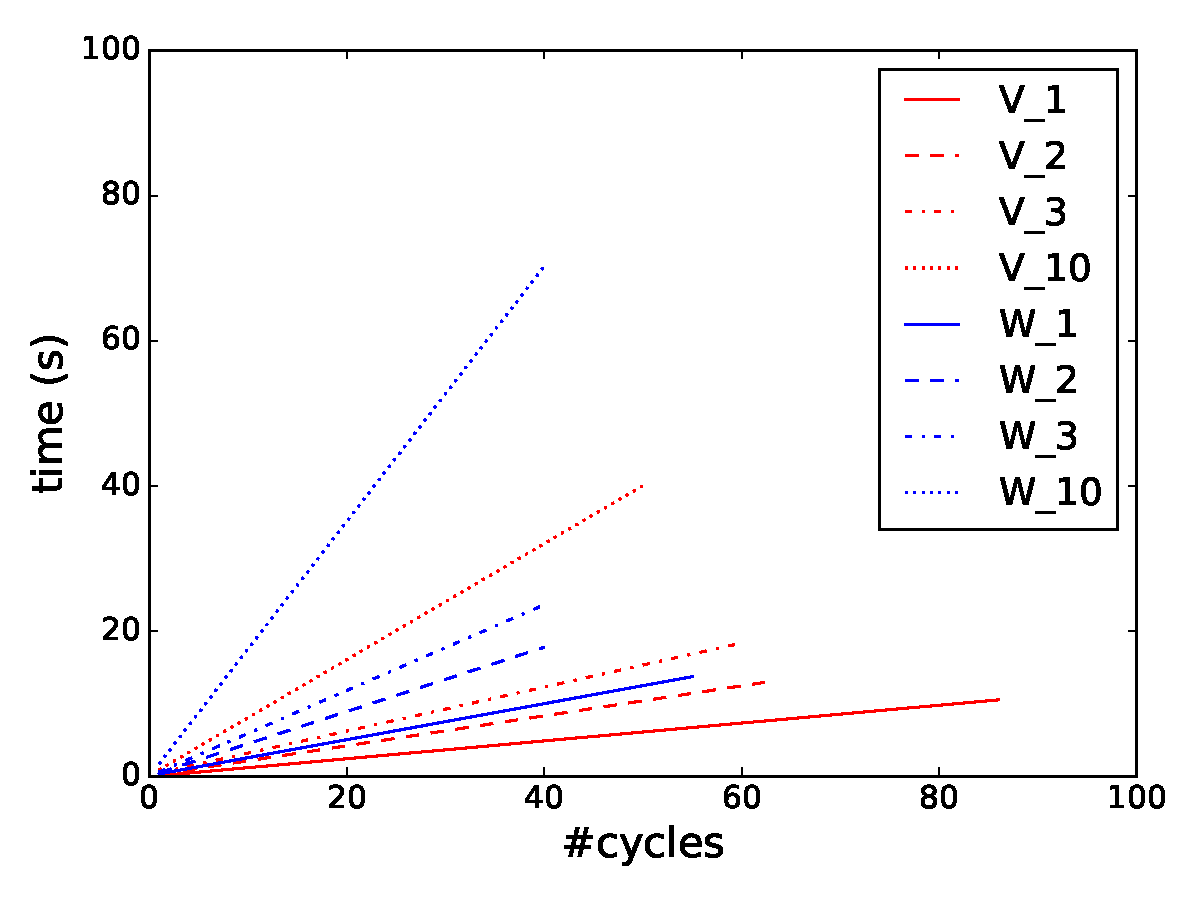
\includegraphics[width=0.4\linewidth]{../ICS/figs/convergence_1_time.pdf}
     \caption{Relative residual norm and execution time as function of number of cycles.}
    \end{figure}
    }
\only<2>{First idea: add more iterations at each level or more complex cycles.
\begin{figure}
    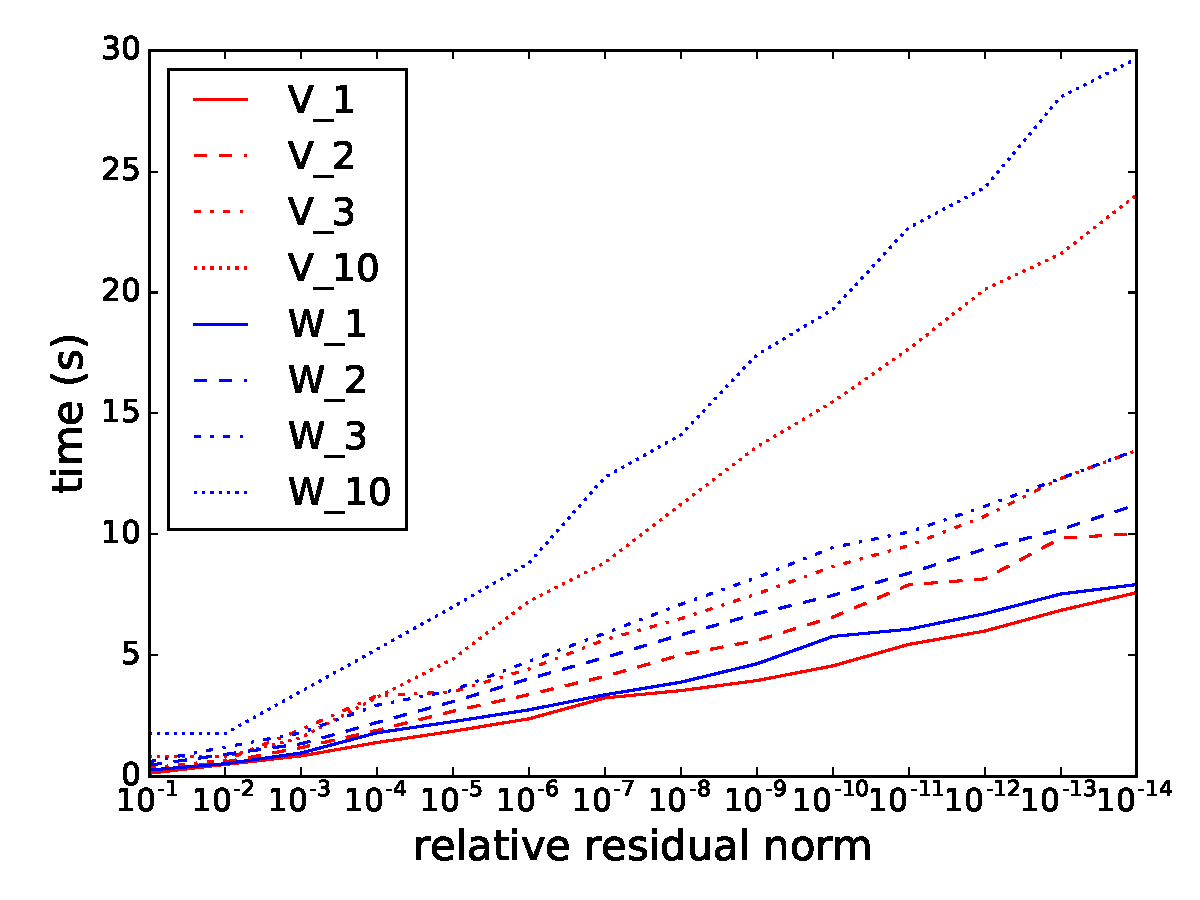
\includegraphics[width=0.5\linewidth]{../ICS/figs/time_convergence.pdf}
     \caption{Relative residual norm as function of execution time.}
\end{figure}
    }
\only<3>{\begin{table}[htb]
 \resizebox{\linewidth}{!}{
 \begin{tabular}{|c|c|c|c|c|c|c|}
  \hline
  Level & \makecell{Matrix \\ size} & \makecell{Non-zero \\ elements} & \makecell{Relax \\ (down)} & \makecell{Relax \\ (up)} & \makecell{Restriction} & \makecell{Interpolation} \\
  \hline
  1 & 512,000 & 4,042,520 & 20 ms & 20 ms & 15 ms & -\\
  \hline
  2 & 256,000 & 6,475,239 & 20 ms & 25 ms & 12 ms & 4 ms\\
  \hline
  3 & 58,893 & 2,000,513 & 8 ms & 8 ms & 3 ms & 2 ms\\
  \hline
  4 & 14,285 & 788,509 & 2 ms & 2 ms & 1 ms & 0.7 ms\\
  \hline
  5 & 4,238 & 386,333 & 1 ms & 1 ms & 0.5 ms & 0.2 ms\\
  \hline
  6 & 609 & 53,493 & $< 0.1$ ms & $< 0.1$ ms & $< 0.1$ ms & $< 0.1$ ms\\
  \hline
  7 & 69 & 2,873 & $< 0.1$ ms & $< 0.1$ ms & $< 0.1$ ms & $< 0.1$ ms\\
  \hline
  8 & 2 & 4 & $< 0.1$ ms & - & - & $< 0.1$ ms\\
  \hline
 \end{tabular}
 }
 \caption{Time breakdown of a V-cycle with $\alpha=1$.}
 \label{table.measures}
\end{table}

$\Rightarrow$ Relaxations represent $\approx66\%$ of the total cost of a V-cycle.}

\end{center}
 
\end{frame}

\begin{frame}{The \textsc{Up}-cycle}
 
 After several tries: the \textsc{Up}-cycle.\\
 We do relaxations only when going up in the V-cycle.
  \begin{figure}
  \centering
 %\resizebox{\linewidth}{4cm}{
 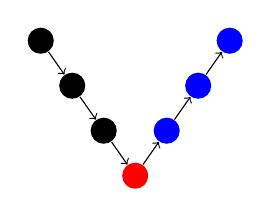
\begin{tikzpicture}
 
 
\begin{scope}[xscale=2/5,yscale=4/7]

    \node[circle,fill=black] (a) at (-3,3) { };
    \node[circle,fill=black] (b) at (-2,2) {};
    \node[circle,fill=black] (c) at (-1,1) {};
    \node[circle,fill=red] (d) at (0,0) {};
    \node[circle,fill=blue] (e) at (1,1) {};
    \node[circle,fill=blue] (f) at (2,2) {};
    \node[circle,fill=blue] (g) at (3,3) {};
    
    \draw[->] (a) -- (b);
    \draw[->] (b) -- (c);
    \draw[->] (c) -- (d);
    \draw[->] (d) -- (e);
    \draw[->] (e) -- (f);
    \draw[->] (f) -- (g);
    \end{scope}

 \end{tikzpicture}
 %}
 \caption{Blue: relaxation. Red: exact solve. Black: nothing.}
 
\end{figure}
 
\end{frame}

\begin{frame}{Results}
\only<1>{
\begin{figure}
    \centering
    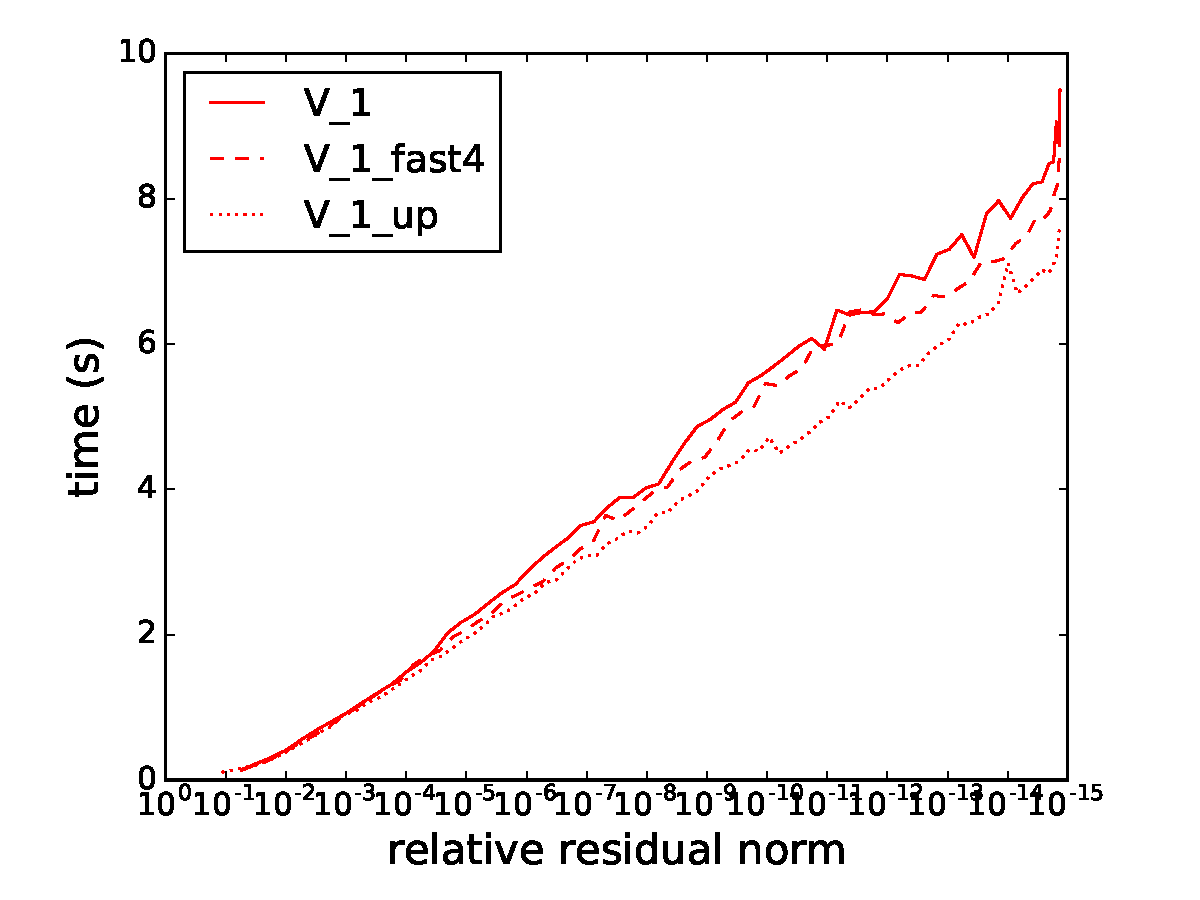
\includegraphics[width=0.4\linewidth]{../ICS/figs/time_convergence_up_1.pdf}
    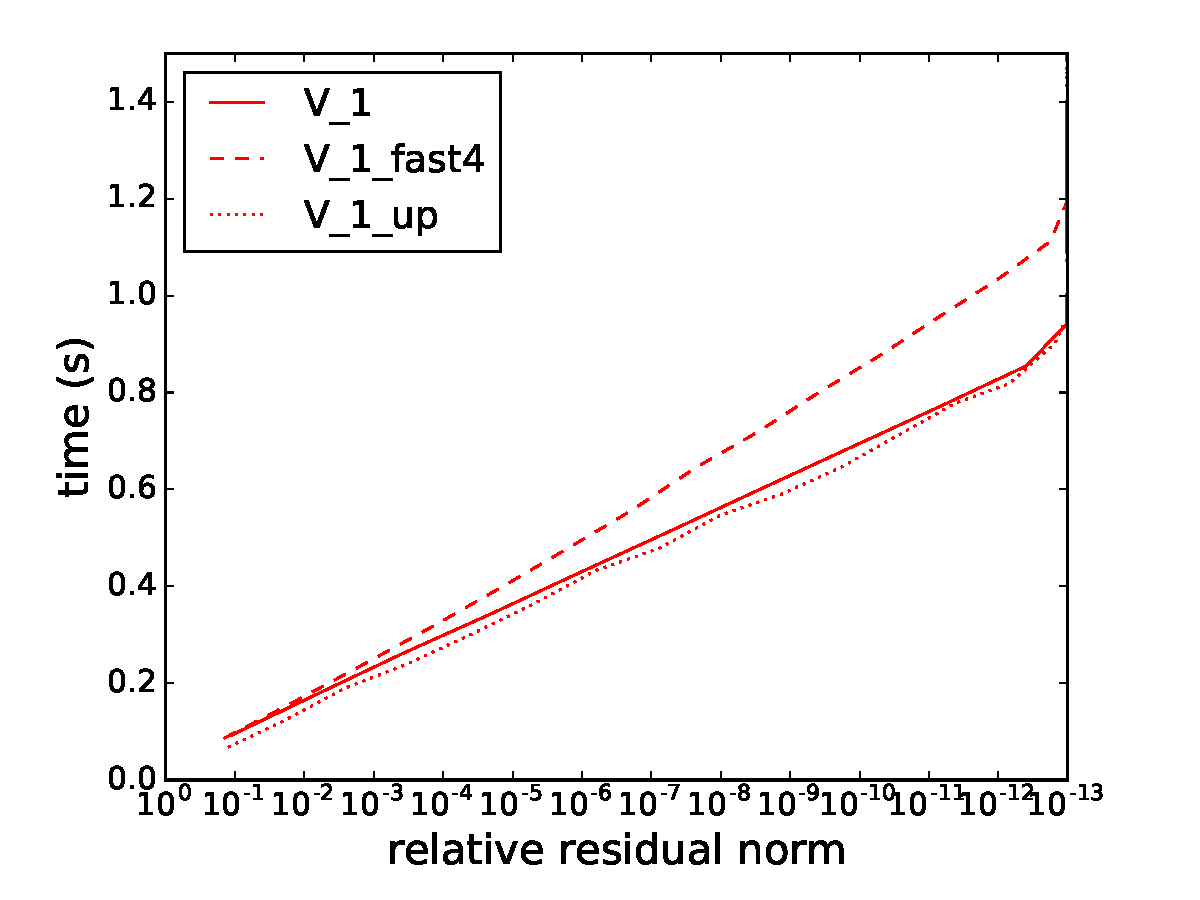
\includegraphics[width=0.4\linewidth]{../ICS/figs/time_convergence_up_2.pdf}\\
    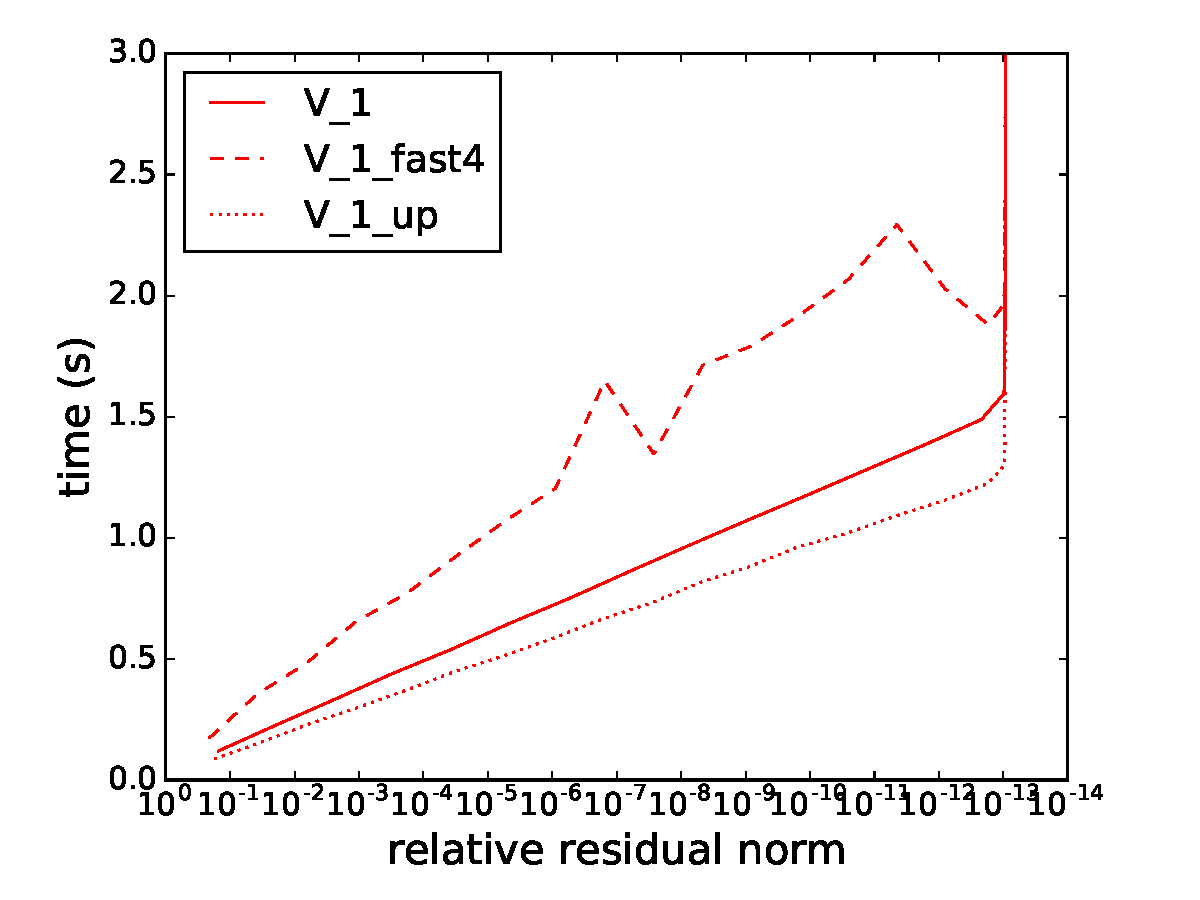
\includegraphics[width=0.4\linewidth]{../ICS/figs/time_convergence_up_3.pdf}
    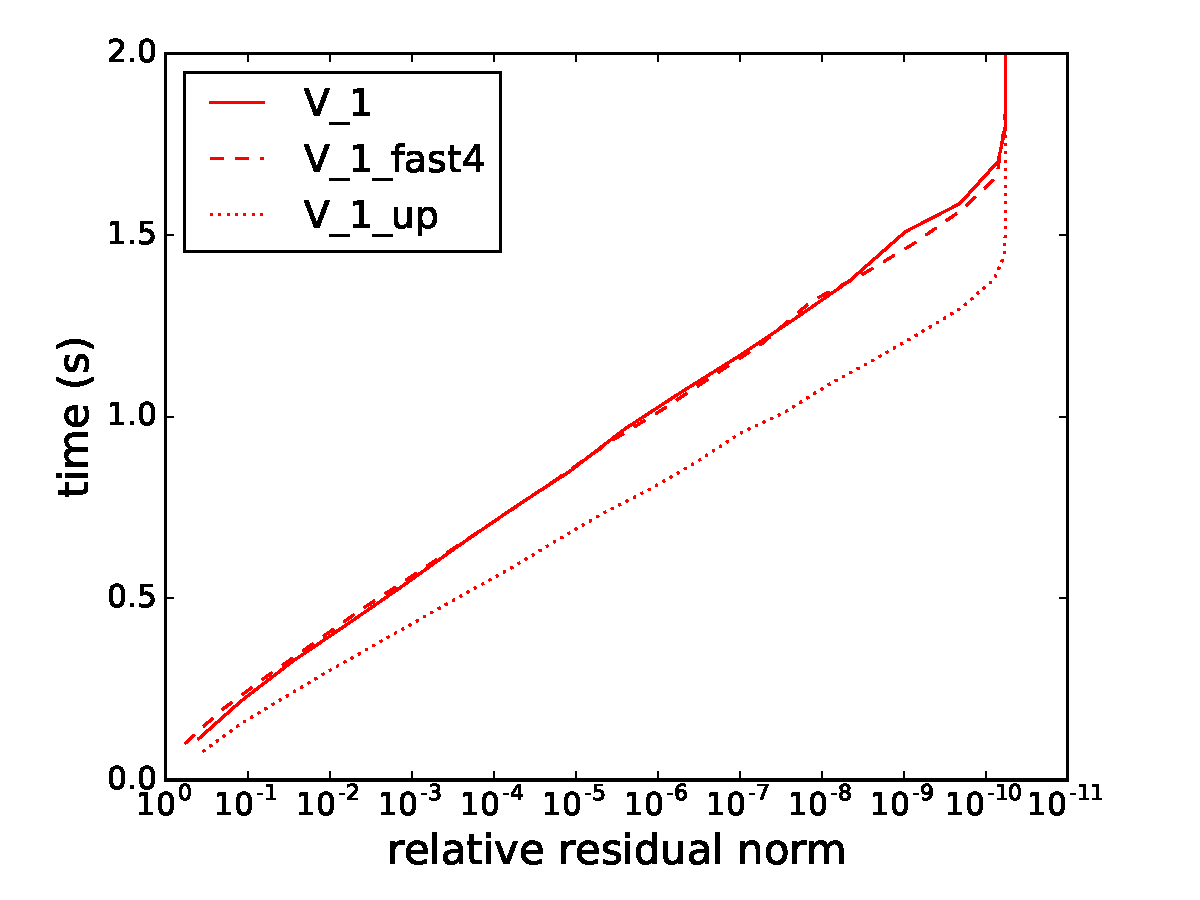
\includegraphics[width=0.4\linewidth]{../ICS/figs/time_convergence_up_4.pdf}
    \label{fig.up_comparison}
\end{figure}}
\only<2>{
\begin{figure}
    \centering
    \subfloat[3x3x3]{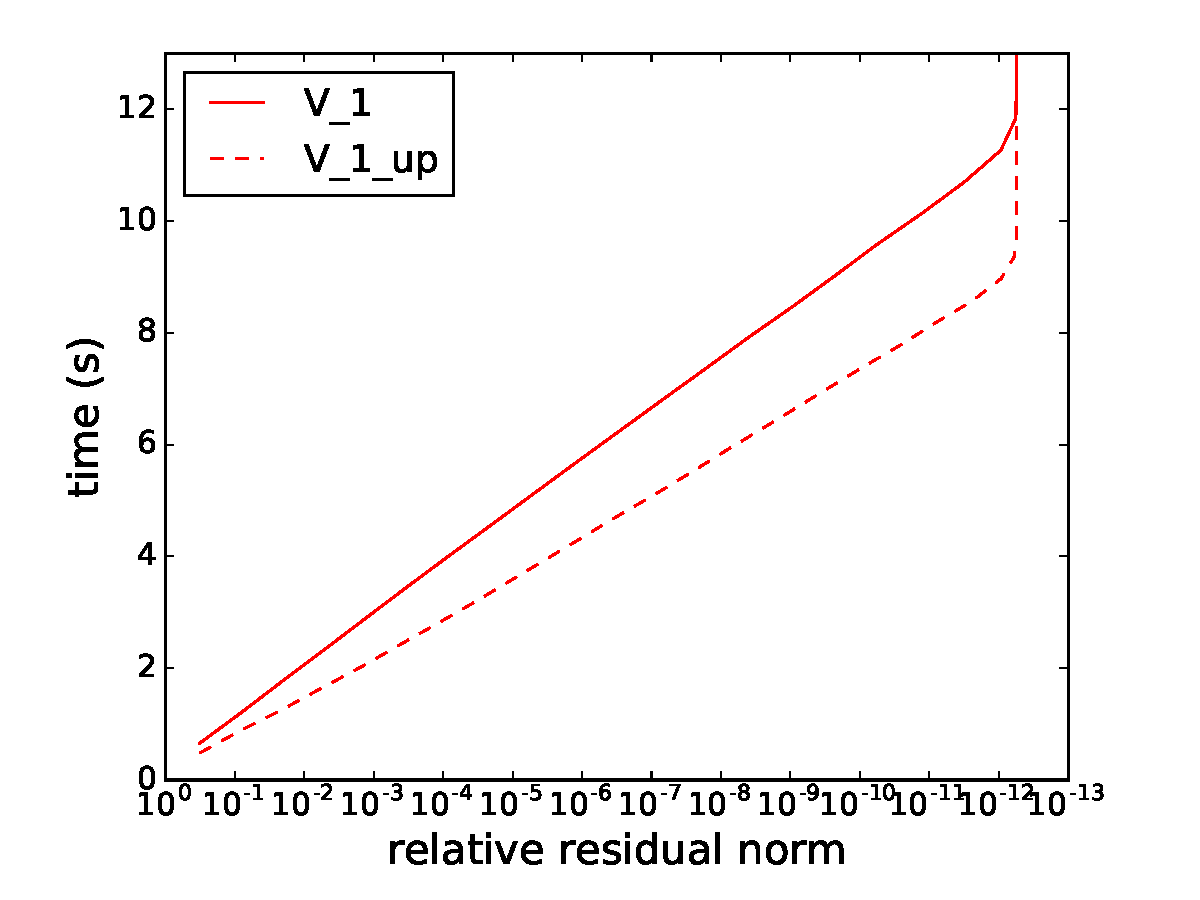
\includegraphics[width=0.33\linewidth]{../ICS/figs/mt_27.pdf}}
    \subfloat[6x6x1]{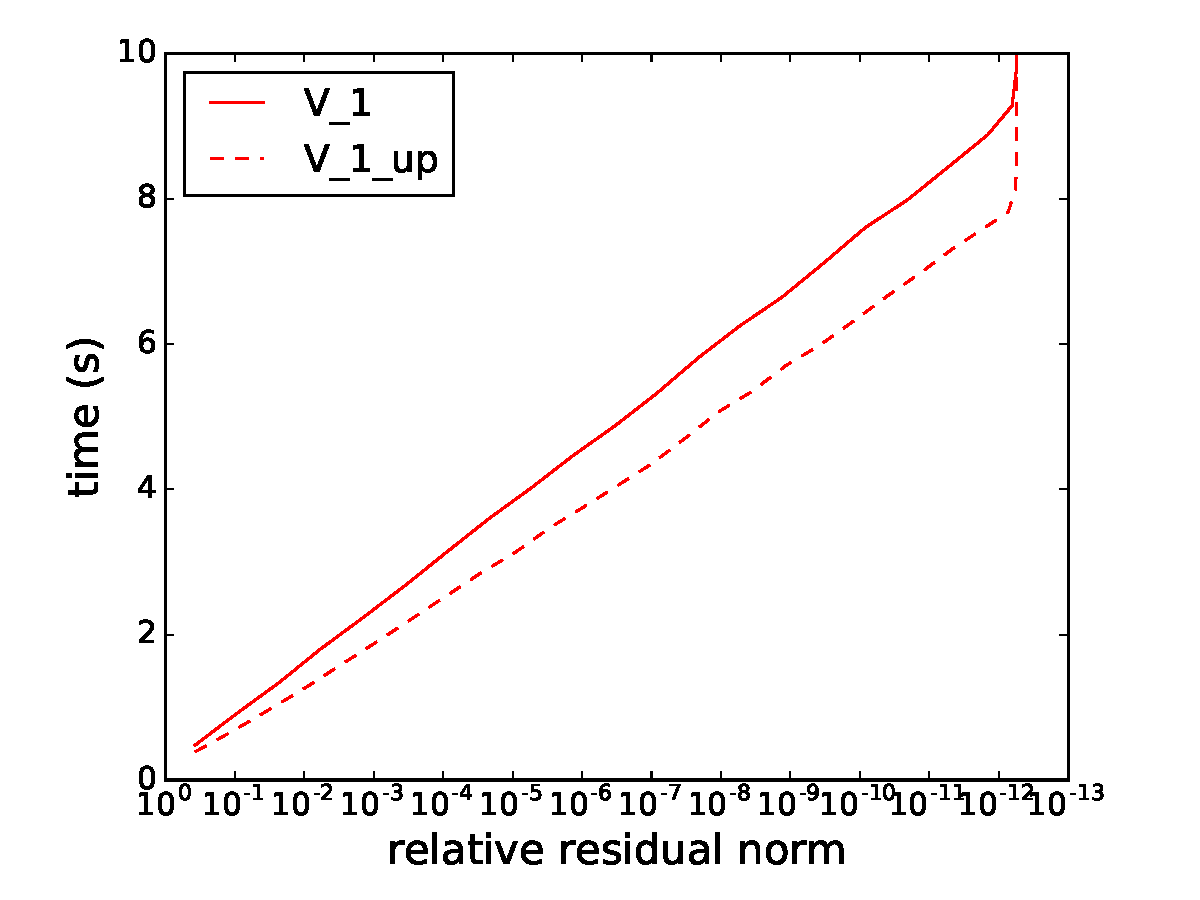
\includegraphics[width=0.33\linewidth]{../ICS/figs/mt_36.pdf}}
    \subfloat[4x4x4]{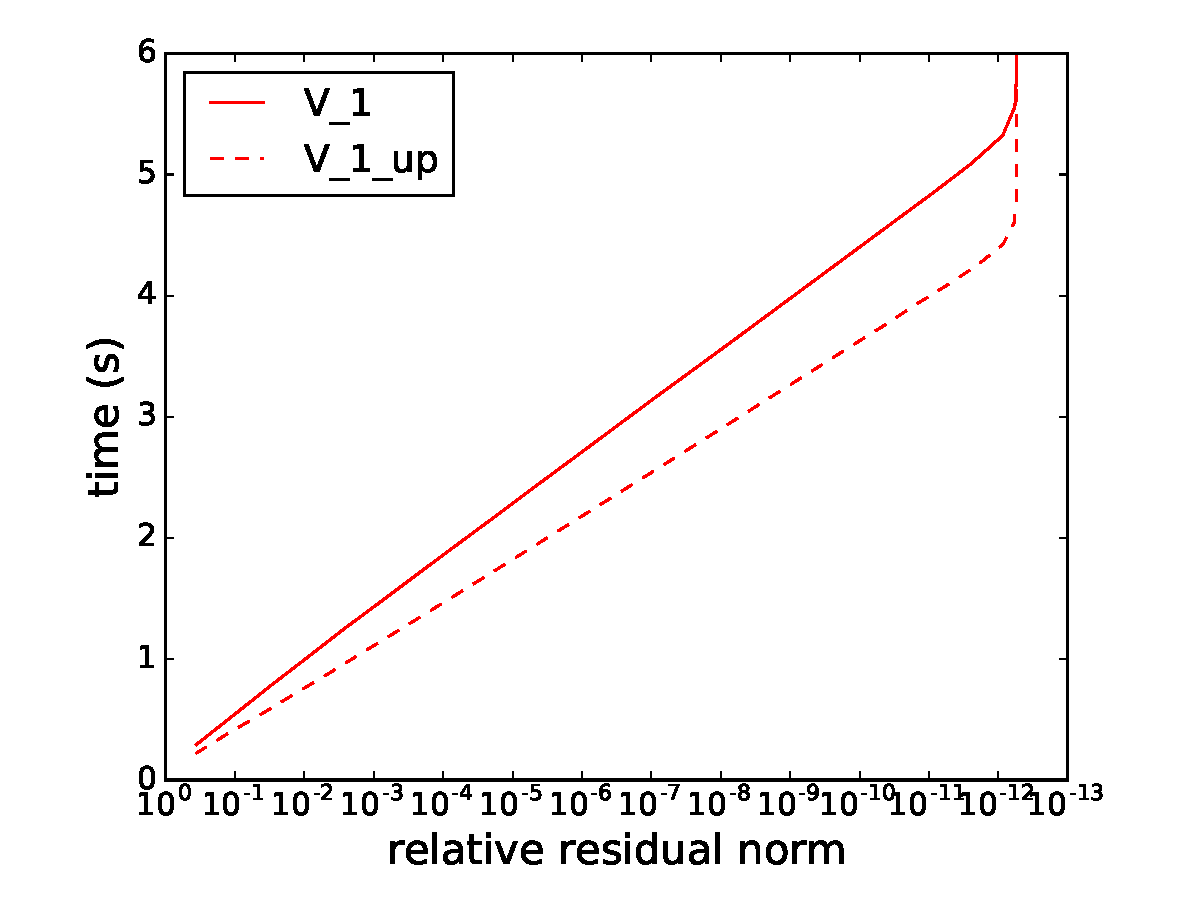
\includegraphics[width=0.33\linewidth]{../ICS/figs/mt_64.pdf}}
    \end{figure}
   
 Overall, between \red{7\% and 28\%} of improvement for reaching max accuracy on our tests. 
    }
 
 
\end{frame}


\section{Bitwidth, performance and accuracy}

\begin{frame}{Outline}
 \tableofcontents[currentsection]
\end{frame}

\begin{frame}{Impact of bitwidth}
 
 \only<1,2,4>{\begin{itemize}
  \item The bitwidth is a hardware limitation: we can't have results accurate to $2^{-1000}$ using double floating-point representation.
  \item However, using a small bitwidth makes computations faster and more energy-efficient~\cite{govindu:2003}.
  \pause
  \item We rewrite the MG algorithm: one version using only single-precision floating-points and one version with the relaxation algorithm using MPFR variables (arbitrary precision)~\cite{MPFR}.
  \pause
  \vspace{0.5cm}
  \item Conclusion: using small bitwidths does not change the convergence rate (until late).
 \end{itemize}}

\only<3>{\begin{figure}[htb]
    \centering
    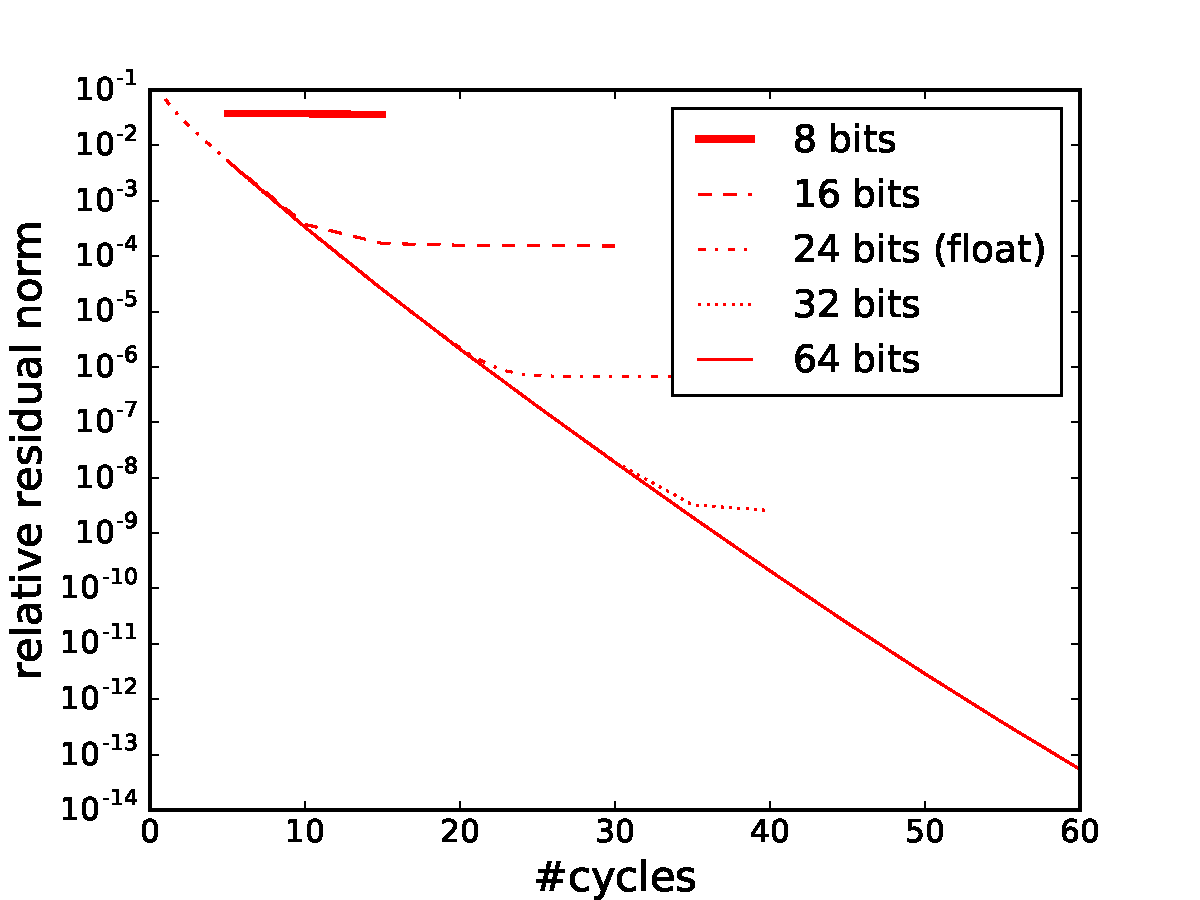
\includegraphics[width=0.7\linewidth]{../ICS/figs/bits_convergence.pdf}
    \caption{Accuracy for different number of \textbf{mantissa} bits.}
%    Points (except for 24 bits) were obtained only for multiples of 5
%    iterations, but it is enough to see the thresholds appear.}
    \label{fig.bits_accuracy}
\end{figure}}
 
\end{frame}

 \begin{frame}{Algorithm}
  $t$ a threshold, $\textsc{Update}(b)$ a function which returns an integer greater than $b$.

   \begin{enumerate}
   \only<1>{\item $b \leftarrow 64$.}
   \only<2>{\item $b \leftarrow {\color{red} 16}$.}
   \item {\textbf{While} \emph{nb\_iters $<$ max\_iter \textbf{and} rel\_res\_norm $>$ tolerance}}
        \begin{enumerate}
	  \item Do a cycle at precision $b$.
	  \item Compute new\_rel\_res\_norm.
	  \only<2>{\item {\color{red} \textbf{If} \emph{new\_rel\_res\_norm $>$ $t \times$rel\_res\_norm} \textbf{Then} $b \leftarrow \textsc{Update}(b)$.}}
	  \item rel\_res\_norm $\leftarrow$ new\_rel\_res\_norm.
	  \item nb\_iters $\leftarrow$ nb\_iters$+1$.
	  \end{enumerate}
   \end{enumerate}
\end{frame}

\begin{frame}{Algorithm}
 
\begin{figure}[htb]
    \centering
    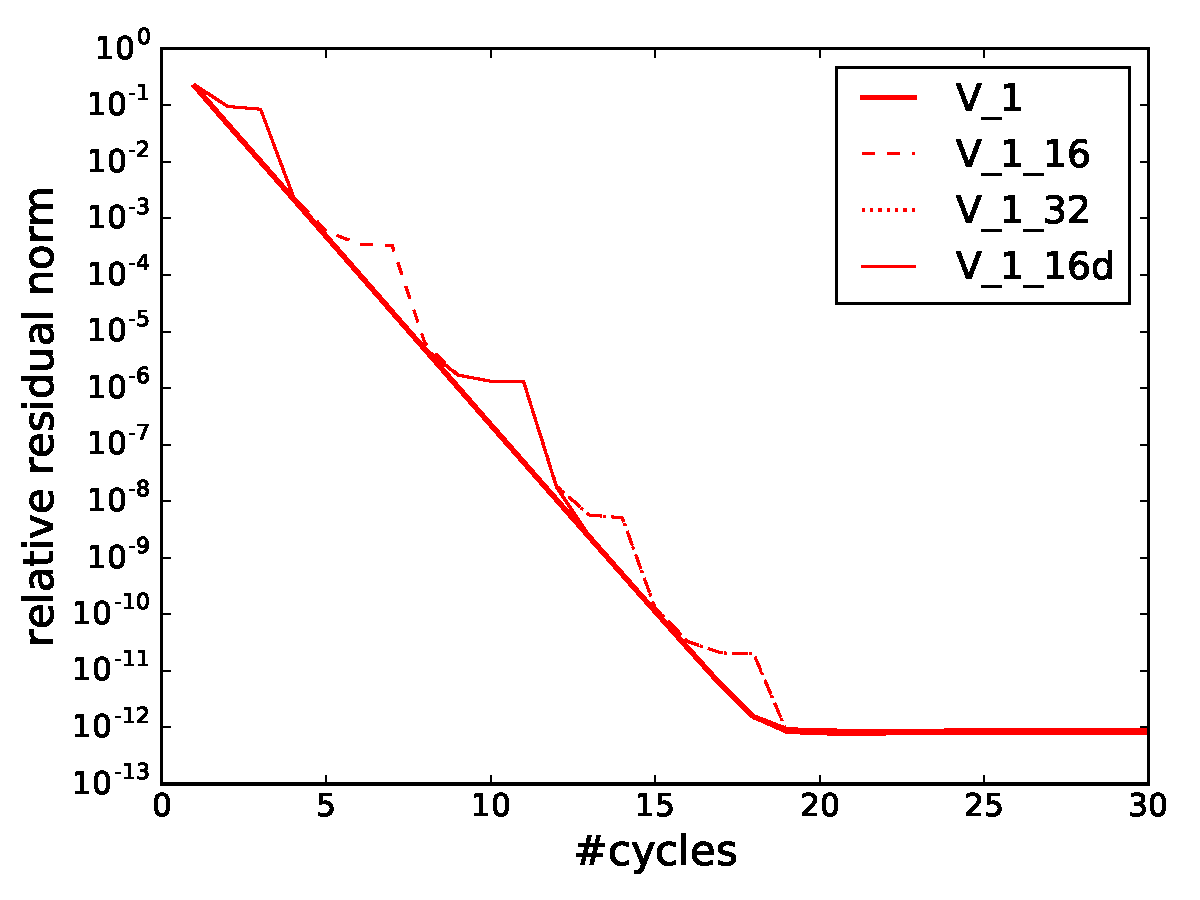
\includegraphics[width=0.7\linewidth]{../ICS/figs/prec_incr.pdf}
    \caption{Accuracy of adaptive algorithms compared to the original
    double-precision with a precision threshold of $0.8$.}
    \label{fig.prec_incr}
\end{figure}
\end{frame}

\begin{frame}{Model}
 How to estimate the benefits in term of execution time ?
 \pause
 \vspace{0.5cm}
 
 \[ Time(n,b) = a\cdot n^3 \cdot b^\alpha + c \]
 
 \begin{itemize}
    \item $n$: size of the problem (we worked on 3D grids so $n^3$ for the size of the matrix).
    \item $b$: number of mantissa bits.
    \item $a,\alpha,c$: constants to determine.
 \end{itemize}
 
 We found \red{$\alpha \approx 0.3$} (sublinear...) using single-precision and double-precision codes.
 
\end{frame}


\begin{frame}{Results}
 
 
\begin{figure}
    \only<1>{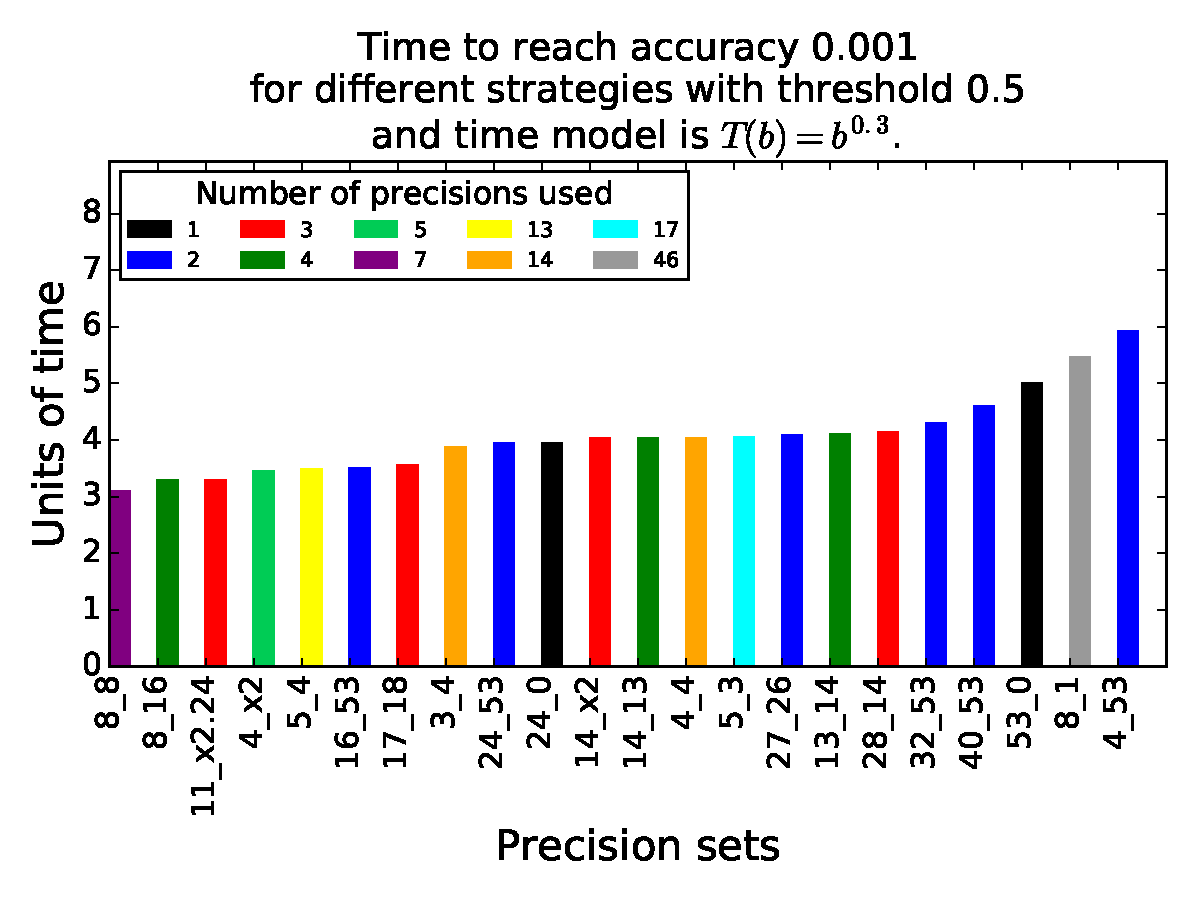
\includegraphics[width=0.6\linewidth]{../ICS/figs/cost_3.pdf}}
    \only<2>{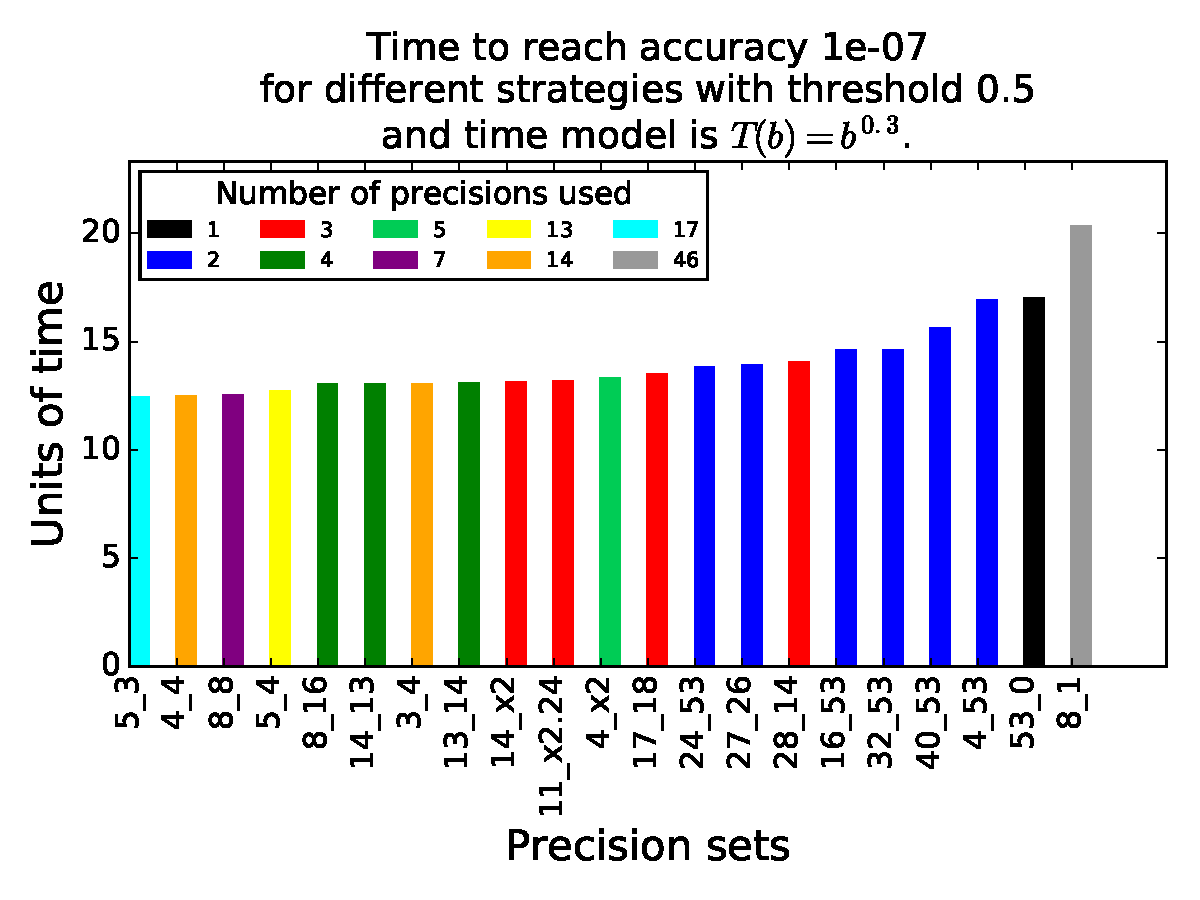
\includegraphics[width=0.6\linewidth]{../ICS/figs/cost_7.pdf}}
    \only<3>{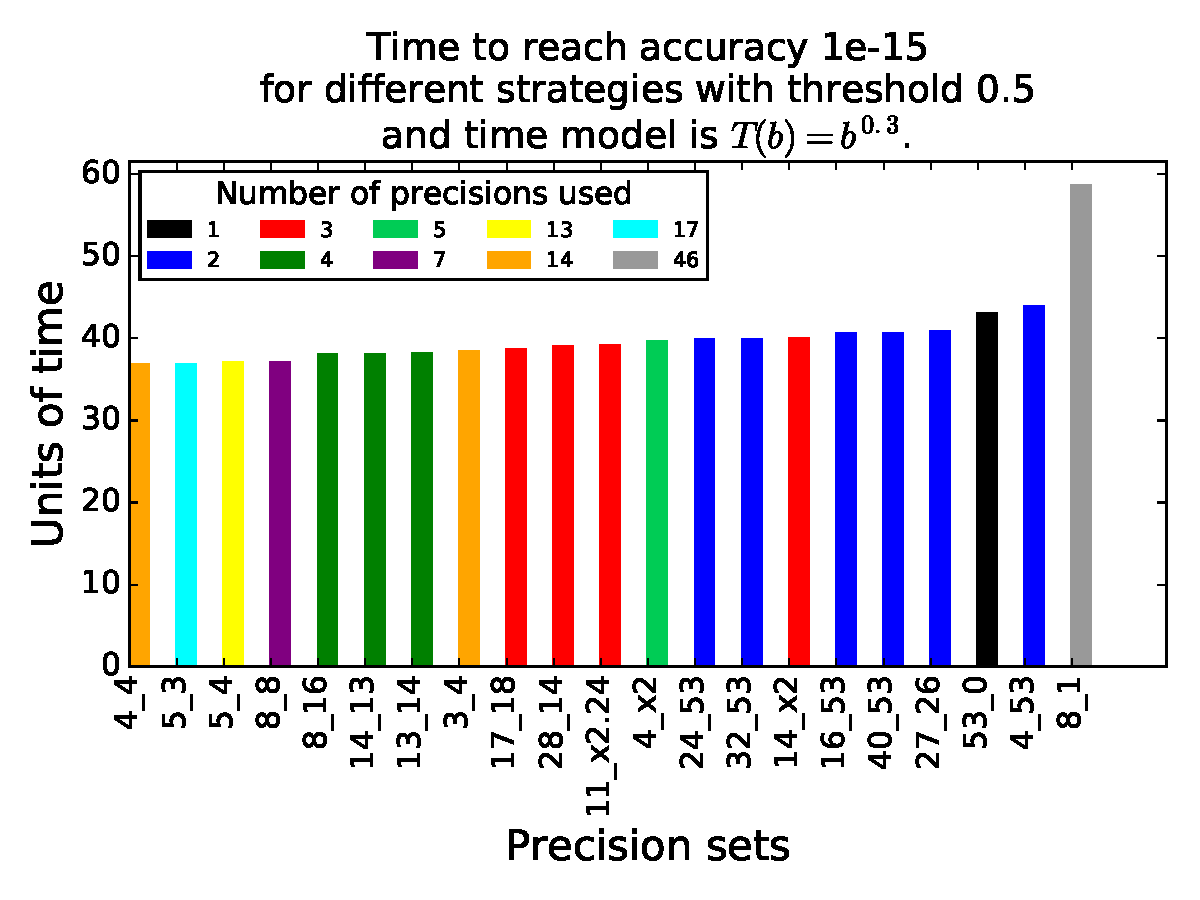
\includegraphics[width=0.6\linewidth]{../ICS/figs/cost_15.pdf}}
    \caption{Cost of the MG solver considering several different dynamic
    precision scenarios to reach accuracy \only<1>{$10^{-3}$}\only<2>{$10^{-7}$}\only<3>{$10^{-15}$}.}
    \label{fig.estimation1}
\end{figure}
 \vspace{-0.5cm}
 GPU compared to double-precision: \red{\only<1>{34}\only<2>{23}\only<3>{9}\%} improvement.
 
\end{frame}

\section{Conclusion}

\begin{frame}{Outline}
 \tableofcontents[currentsection]
\end{frame}

\begin{frame}{Conclusion (1)}

  Final results:
 \begin{itemize}
  \item A new cycle shape that tends to converge faster: the \textsc{Up}-cycle.
  \item A new algorithm for \textit{any} MG cycle shape that reduces execution time and energy consumption.
  \item Up to 30\% expected improvement on a GPU with half-precision/single-precision/double-precision available by mixing \textsc{Up}-cycle and changing bitwidths.
  \item At least 15\% expected improvement for reaching maximum accuracy compared to previously.
 \end{itemize}
 
\end{frame}

\begin{frame}{Conclusion (2)}
 
 Future ideas:
 \begin{itemize}
  \item Model (or measure) the gains in energy consumption instead of execution time.
  \item Change precision \textbf{inside} a cycle?
  \item Link to silent data corruption: what if the environment forces us to work at $10^{-x}$ as max accuracy because of bitflips?
 \end{itemize}

 \pause
 \vspace{0.8cm}
 \begin{center}
  \Large
    Thank you for your attention. Any question?
 \end{center}

 
\end{frame}

\begin{frame}{References}
\bibliography{biblio}
\bibliographystyle{plain}
\end{frame}


\begin{frame}{Grids}

  \begin{tikzpicture}
      \draw[-] (0,-1) -- (0,5) ;
      \draw[-] (1,-1) -- (1,5) ;
      \draw[-] (2,-1) -- (2,5) ;
      \draw[-] (3,-1) -- (3,5) ;
      \draw[-] (4,-1) -- (4,5) ;
      \draw[-] (-1,0) -- (5,0) ;
      \draw[-] (-1,1) -- (5,1) ;
      \draw[-] (-1,2) -- (5,2) ;
      \draw[-] (-1,3) -- (5,3) ;
      \draw[-] (-1,4) -- (5,4) ;
      \foreach \x in {0,1,2,3,4}
    \foreach \y in {0,1,2,3,4}
      {
        \fill (\x,\y) circle (0.1cm);
      }
      \only<1>{
      \foreach \x in {0,1,2,3,4}
    \foreach \y in {0,1,2,3,4}
      {
        \fill[red] (\x,\y) circle (0.09cm);
      }}
      \only<2>{
      \foreach \x in {0,2,4}
    \foreach \y in {0,2,4}
      {
        \fill[red] (\x,\y) circle (0.09cm);
      }
      }
      \only<3>{
      \foreach \x in {0,4}
    \foreach \y in {0,4}
      {
        \fill[red] (\x,\y) circle (0.09cm);
      }
      }
  \end{tikzpicture}
  \hspace{1cm}
  \begin{tikzpicture}
      \draw[-] (0,-1) -- (0,5) ;
    \foreach \y in {0,1,2,3,4}
      {
        \fill (0,\y) circle (0.1cm);
      }
      \only<1>{
    \foreach \y in {0,1,2,3,4}
      {
        \fill[red] (0,\y) circle (0.09cm);
      }}
      \only<2>{
    \foreach \y in {0,2,4}
      {
        \fill[red] (0,\y) circle (0.09cm);
      }
      }
      \only<3>{
    \foreach \y in {0,4}
      {
        \fill[red] (0,\y) circle (0.09cm);
      }
      }
  \end{tikzpicture}

 
\end{frame}
\end{document}
